\section{Resultados}
Se entrenaron los modelos clásicos y basados en redes neuronales con los vectores de comparación diarios. El vector diario obtenido a partir de la ecuación \ref{eq:diff} es denominado diff y el vector obtenido a partir de la ecuación \ref{eq:ratio} se denomina ratio. Para los modelos clásicos se obtuvieron mejores metricas cuando se utiliza como vector de entrada los valores que se encuentran entre las 7 y 20 horas. En cambio, para los modelos basados en redes neuronales se obtienen mejores resultados utilizando los 24 valores diarios.

En las tablas \ref{table:noroeste_accuracy}, \ref{table:noreste_accuracy}, \ref{table:suroeste_accuracy} y \ref{table:sureste2_accuracy} se muestran las metricas de accuracy para todos los modelos de clasificación implementados.

\begin{table}[H]
	\centering
	\hspace{-1cm}
	\begin{subtable}[H]{0.47\linewidth}
		\centering
		\changefontsizes{6pt}
		\begin{tabular}{lrrrr} \hline
			\textbf{Modelo}    & \textbf{diff GHI}      & \textbf{diff RS}       & \textbf{ratio GHI}     & \textbf{ratio RS}      \\ \hline
			SVM                & 0.71                   & 0.72                   & 0.72                   & 0.73                   \\
			KNN                & 0.81                   & 0.79                   & 0.71                   & 0.70                   \\
			Bosques aleatorios & 0.77                   & \textbf{\folder{0.82}} & 0.77                   & 0.80                   \\
			Naive Gaussiano    & 0.66                   & 0.68                   & 0.68                   & 0.67                   \\
			Árbol de decisión  & 0.73                   & 0.75                   & 0.72                   & 0.77                   \\
			Perceptron         & 0.62                   & 0.74                   & 0.74                   & 0.71                   \\
			CNN                & \textbf{\folder{0.82}} & 0.81                   & \textbf{\folder{0.85}} & \textbf{\folder{0.85}} \\
			LSTM               & 0.73                   & 0.79                   & 0.77                   & 0.79                   \\
			RNN                & 0.78                   & 0.69                   & 0.76                   & 0.76                   \\
			Bi LSTM            & 0.74                   & 0.81                   & 0.80                   & 0.84                   \\
			Attention CNN      & 0.43                   & 0.42                   & 0.82                   & 0.82                   \\
			Votación           & 0.74                   & 0.79                   & 0.82                   & \textbf{\folder{0.85}} \\ \hline
		\end{tabular}
		\changefontsizes{10pt}
		\caption{Estacion Noroeste.}
		\label{table:noroeste_accuracy}
	\end{subtable}
	\hspace{1.2cm}
	\begin{subtable}[H]{0.47\linewidth}
		\centering
		\changefontsizes{6pt}
		\begin{tabular}{lrrrr} \hline
			\textbf{Modelo}    & \textbf{diff GHI}      & \textbf{diff RS}       & \textbf{ratio GHI}     & \textbf{ratio RS}      \\ \hline
			SVM                & 0.80                   & 0.80                   & 0.80                   & 0.81                   \\
			KNN                & 0.78                   & 0.79                   & 0.78                   & 0.78                   \\
			Bosques aleatorios & \textbf{\folder{0.84}} & \textbf{\folder{0.85}} & 0.83                   & \textbf{\folder{0.88}} \\
			Naive Gaussiano    & 0.69                   & 0.70                   & 0.77                   & 0.78                   \\
			Árbol de decisión  & 0.78                   & 0.75                   & 0.79                   & 0.82                   \\
			Perceptron         & 0.66                   & 0.70                   & 0.81                   & 0.84                   \\
			CNN                & \textbf{\folder{0.84}} & 0.81                   & 0.82                   & 0.84                   \\
			LSTM               & 0.81                   & \textbf{\folder{0.85}} & 0.76                   & 0.82                   \\
			RNN                & 0.73                   & 0.79                   & 0.81                   & 0.81                   \\
			Bi LSTM            & 0.77                   & 0.80                   & \textbf{\folder{0.84}} & 0.83                   \\
			Attention CNN      & 0.48                   & 0.48                   & 0.81                   & 0.83                   \\
			Votación           & 0.77                   & 0.80                   & 0.81                   & 0.83                   \\ \hline
		\end{tabular}
		\changefontsizes{10pt}
		\caption{Estacion Noreste.}
		\label{table:noreste_accuracy}
	\end{subtable}
	\hspace*{-1cm}
	\begin{subtable}[H]{0.47\linewidth}
		\centering
		\changefontsizes{6pt}
		\begin{tabular}{lrrrr} \hline
			\textbf{Modelo}    & \textbf{diff GHI}      & \textbf{diff RS}       & \textbf{ratio GHI}     & \textbf{ratio RS}      \\ \hline
			SVM                & 0.74                   & 0.75                   & 0.75                   & 0.75                   \\
			KNN                & 0.75                   & 0.76                   & 0.70                   & 0.69                   \\
			Bosques aleatorios & 0.81                   & 0.83                   & \textbf{\folder{0.83}} & 0.83                   \\
			Naive Gaussiano    & 0.69                   & 0.67                   & 0.71                   & 0.70                   \\
			Árbol de decisión  & 0.76                   & 0.75                   & 0.77                   & 0.75                   \\
			Perceptron         & 0.65                   & 0.70                   & 0.74                   & 0.73                   \\
			CNN                & \textbf{\folder{0.85}} & \textbf{\folder{0.84}} & 0.82                   & 0.83                   \\
			LSTM               & 0.74                   & 0.76                   & 0.80                   & 0.83                   \\
			RNN                & 0.74                   & 0.75                   & 0.81                   & \textbf{\folder{0.84}} \\
			Bi LSTM            & 0.72                   & 0.81                   & 0.79                   & \textbf{\folder{0.84}} \\
			Attention CNN      & 0.42                   & 0.42                   & 0.82                   & 0.82                   \\
			Votación           & 0.74                   & 0.76                   & 0.82                   & 0.83                   \\  \hline
		\end{tabular}
		\changefontsizes{10pt}
		\caption{Estacion Suroeste.}
		\label{table:suroeste_accuracy}
	\end{subtable}
	\hspace{1.2cm}
	\begin{subtable}[H]{0.47\linewidth}
		\centering
		\changefontsizes{6pt}
		\begin{tabular}{lrrrr} \hline
			\textbf{Modelo}    & \textbf{diff GHI}      & \textbf{diff RS}       & \textbf{ratio GHI}     & \textbf{ratio RS}      \\ \hline
			SVM                & 0.73                   & 0.76                   & 0.77                   & 0.81                   \\
			KNN                & 0.76                   & 0.81                   & 0.70                   & 0.67                   \\
			Bosques aleatorios & 0.82                   & \textbf{\folder{0.84}} & 0.82                   & 0.83                   \\
			Naive Gaussiano    & 0.67                   & 0.71                   & 0.71                   & 0.70                   \\
			Árbol de decisión  & 0.71                   & 0.80                   & 0.75                   & 0.79                   \\
			Perceptron         & 0.50                   & 0.64                   & 0.76                   & 0.80                   \\
			CNN                & \textbf{\folder{0.86}} & 0.80                   & \textbf{\folder{0.84}} & \textbf{\folder{0.86}} \\
			LSTM               & 0.71                   & 0.79                   & 0.78                   & 0.83                   \\
			RNN                & 0.80                   & 0.79                   & 0.80                   & 0.82                   \\
			Bi LSTM            & 0.72                   & 0.80                   & 0.80                   & 0.84                   \\
			Attention CNN      & 0.47                   & 0.47                   & 0.82                   & 0.83                   \\
			Votación           & 0.72                   & 0.79                   & 0.80                   & 0.83                   \\ \hline
		\end{tabular}
		\changefontsizes{10pt}
		\caption{Estacion Sureste 2.}
		\label{table:sureste2_accuracy}
	\end{subtable}
	\caption{Accuracy obtenido por los diferentes modelos de clasificación para las estaciones seleccionadas con base a los diferentes tipos de comparación.}
\end{table}
Se seleccionaron aleatoriamente una fecha por estación para probar los modelos. En la figura \ref{fig:test_daily} se muestran las fechas seleccionados.
\begin{figure}[H]
	\centering
	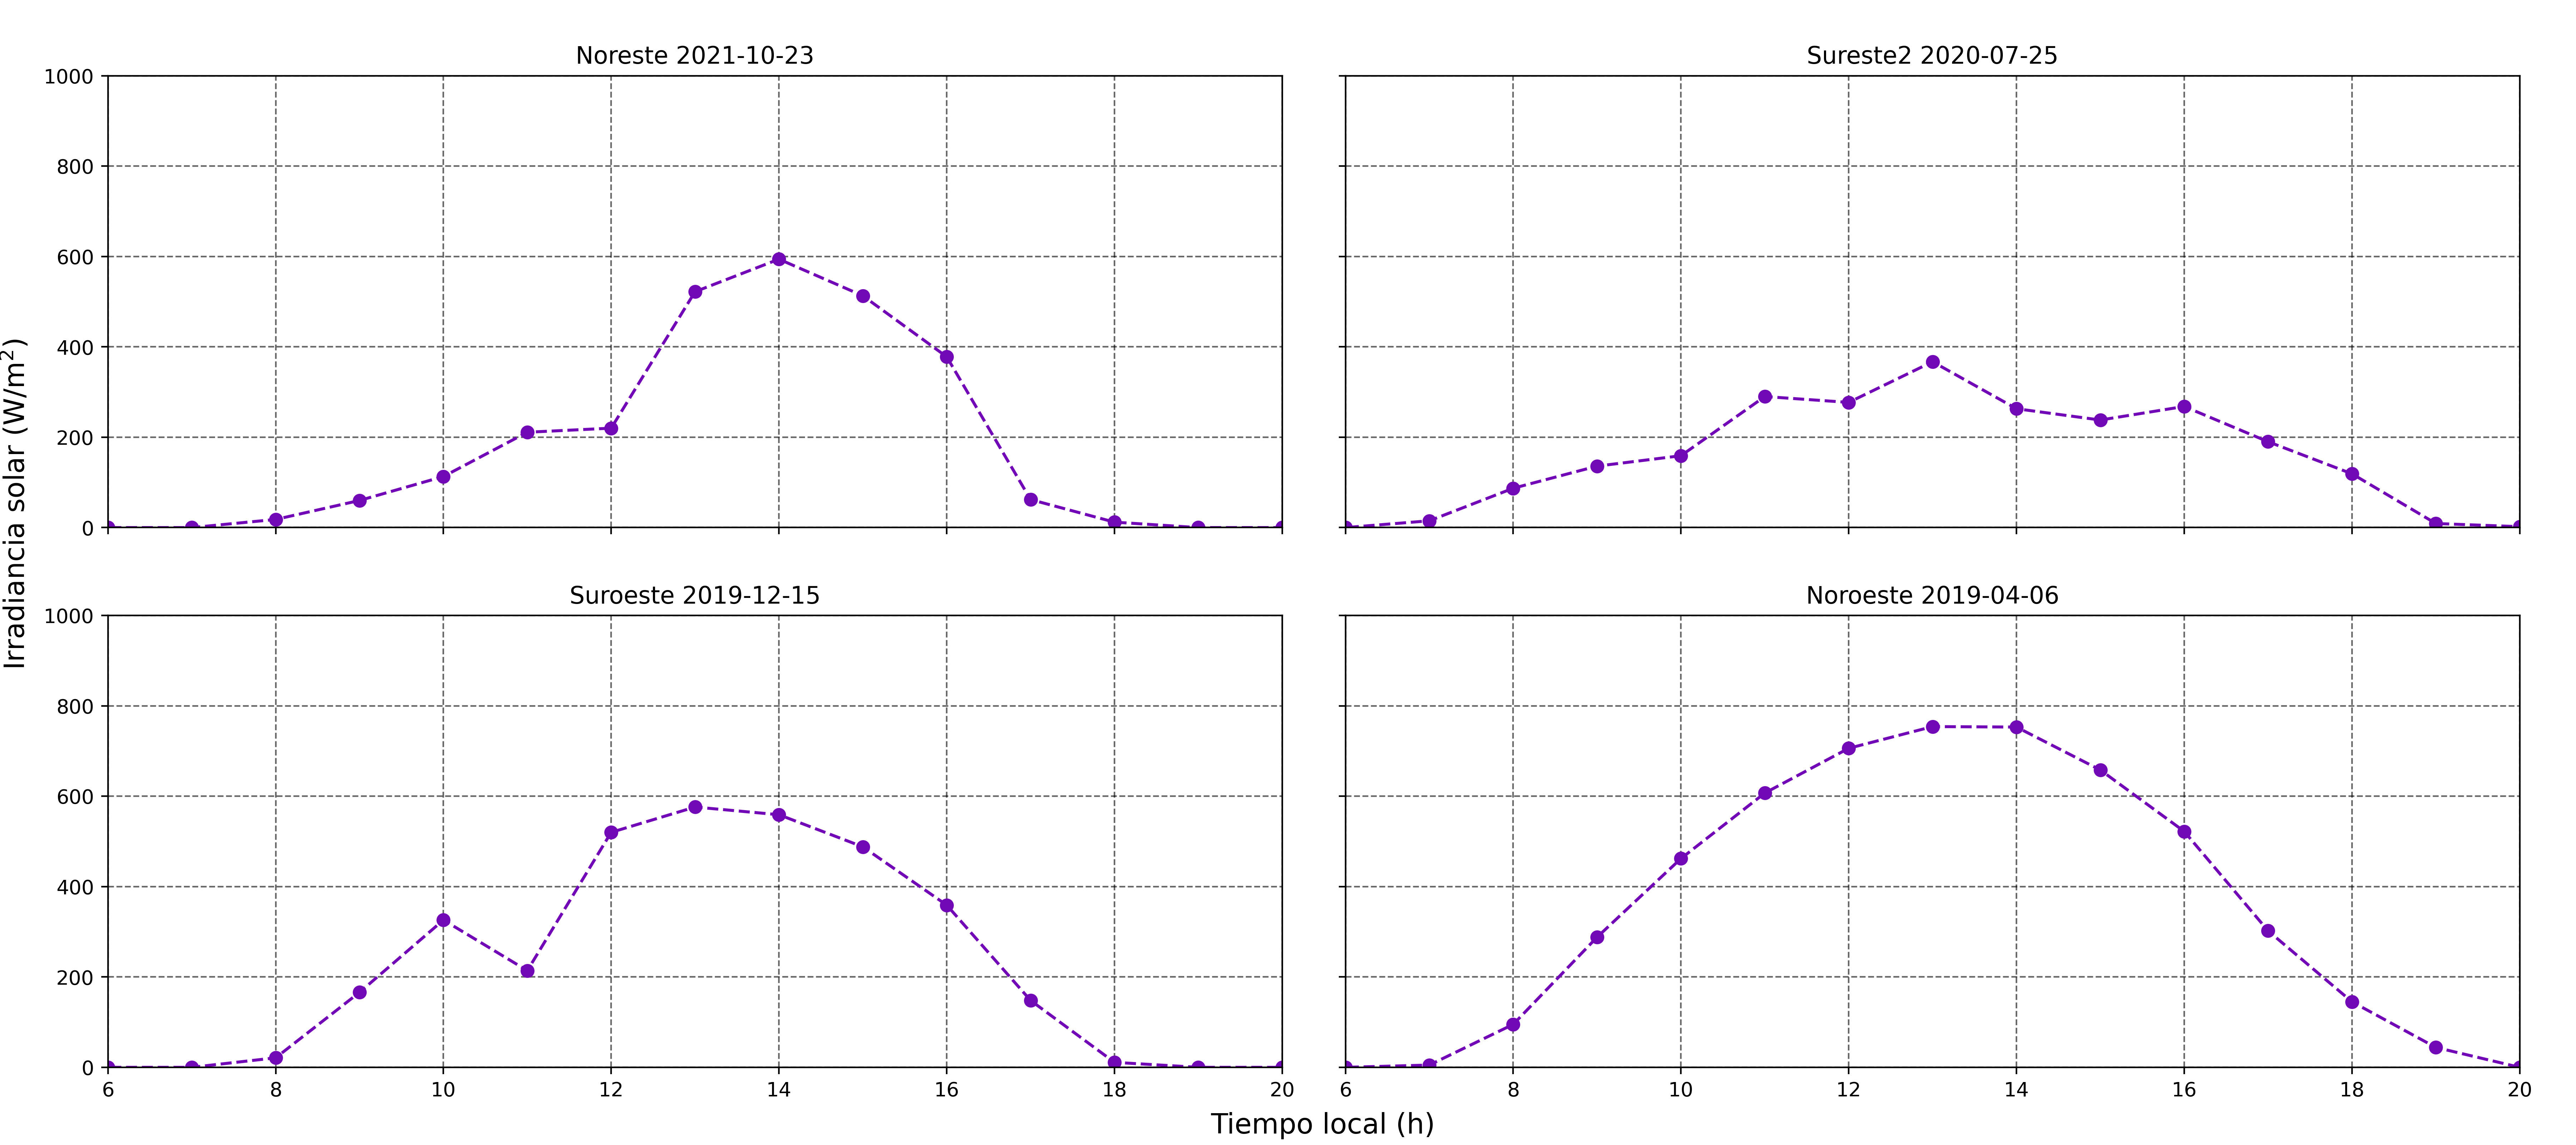
\includegraphics[width=14cm]{Graphics/test_daily.png}
	\caption{Fechas de la base de datos elegidos aleatoriamente.}
	\label{fig:test_daily}
\end{figure}
El modelo de arboles de decisión fallo con la medición de la estación Noreste, este lo clasificó como parcialmente nublado. Los modelos de Perceptron y SVM fallaron con la medición de la estación Noroeste, clasificando este día como parcialmente nublado. En las demás fechas, los modelos clasificaron de forma correcta a las mediciones tomadas aleatoriamente. En la figura \ref{fig:test_models} se muestran los resultados de las clasificaciones de los modelos implementados para las fechas mostradas en la figura \ref{fig:test_daily}
\begin{figure}[H]
	\centering
	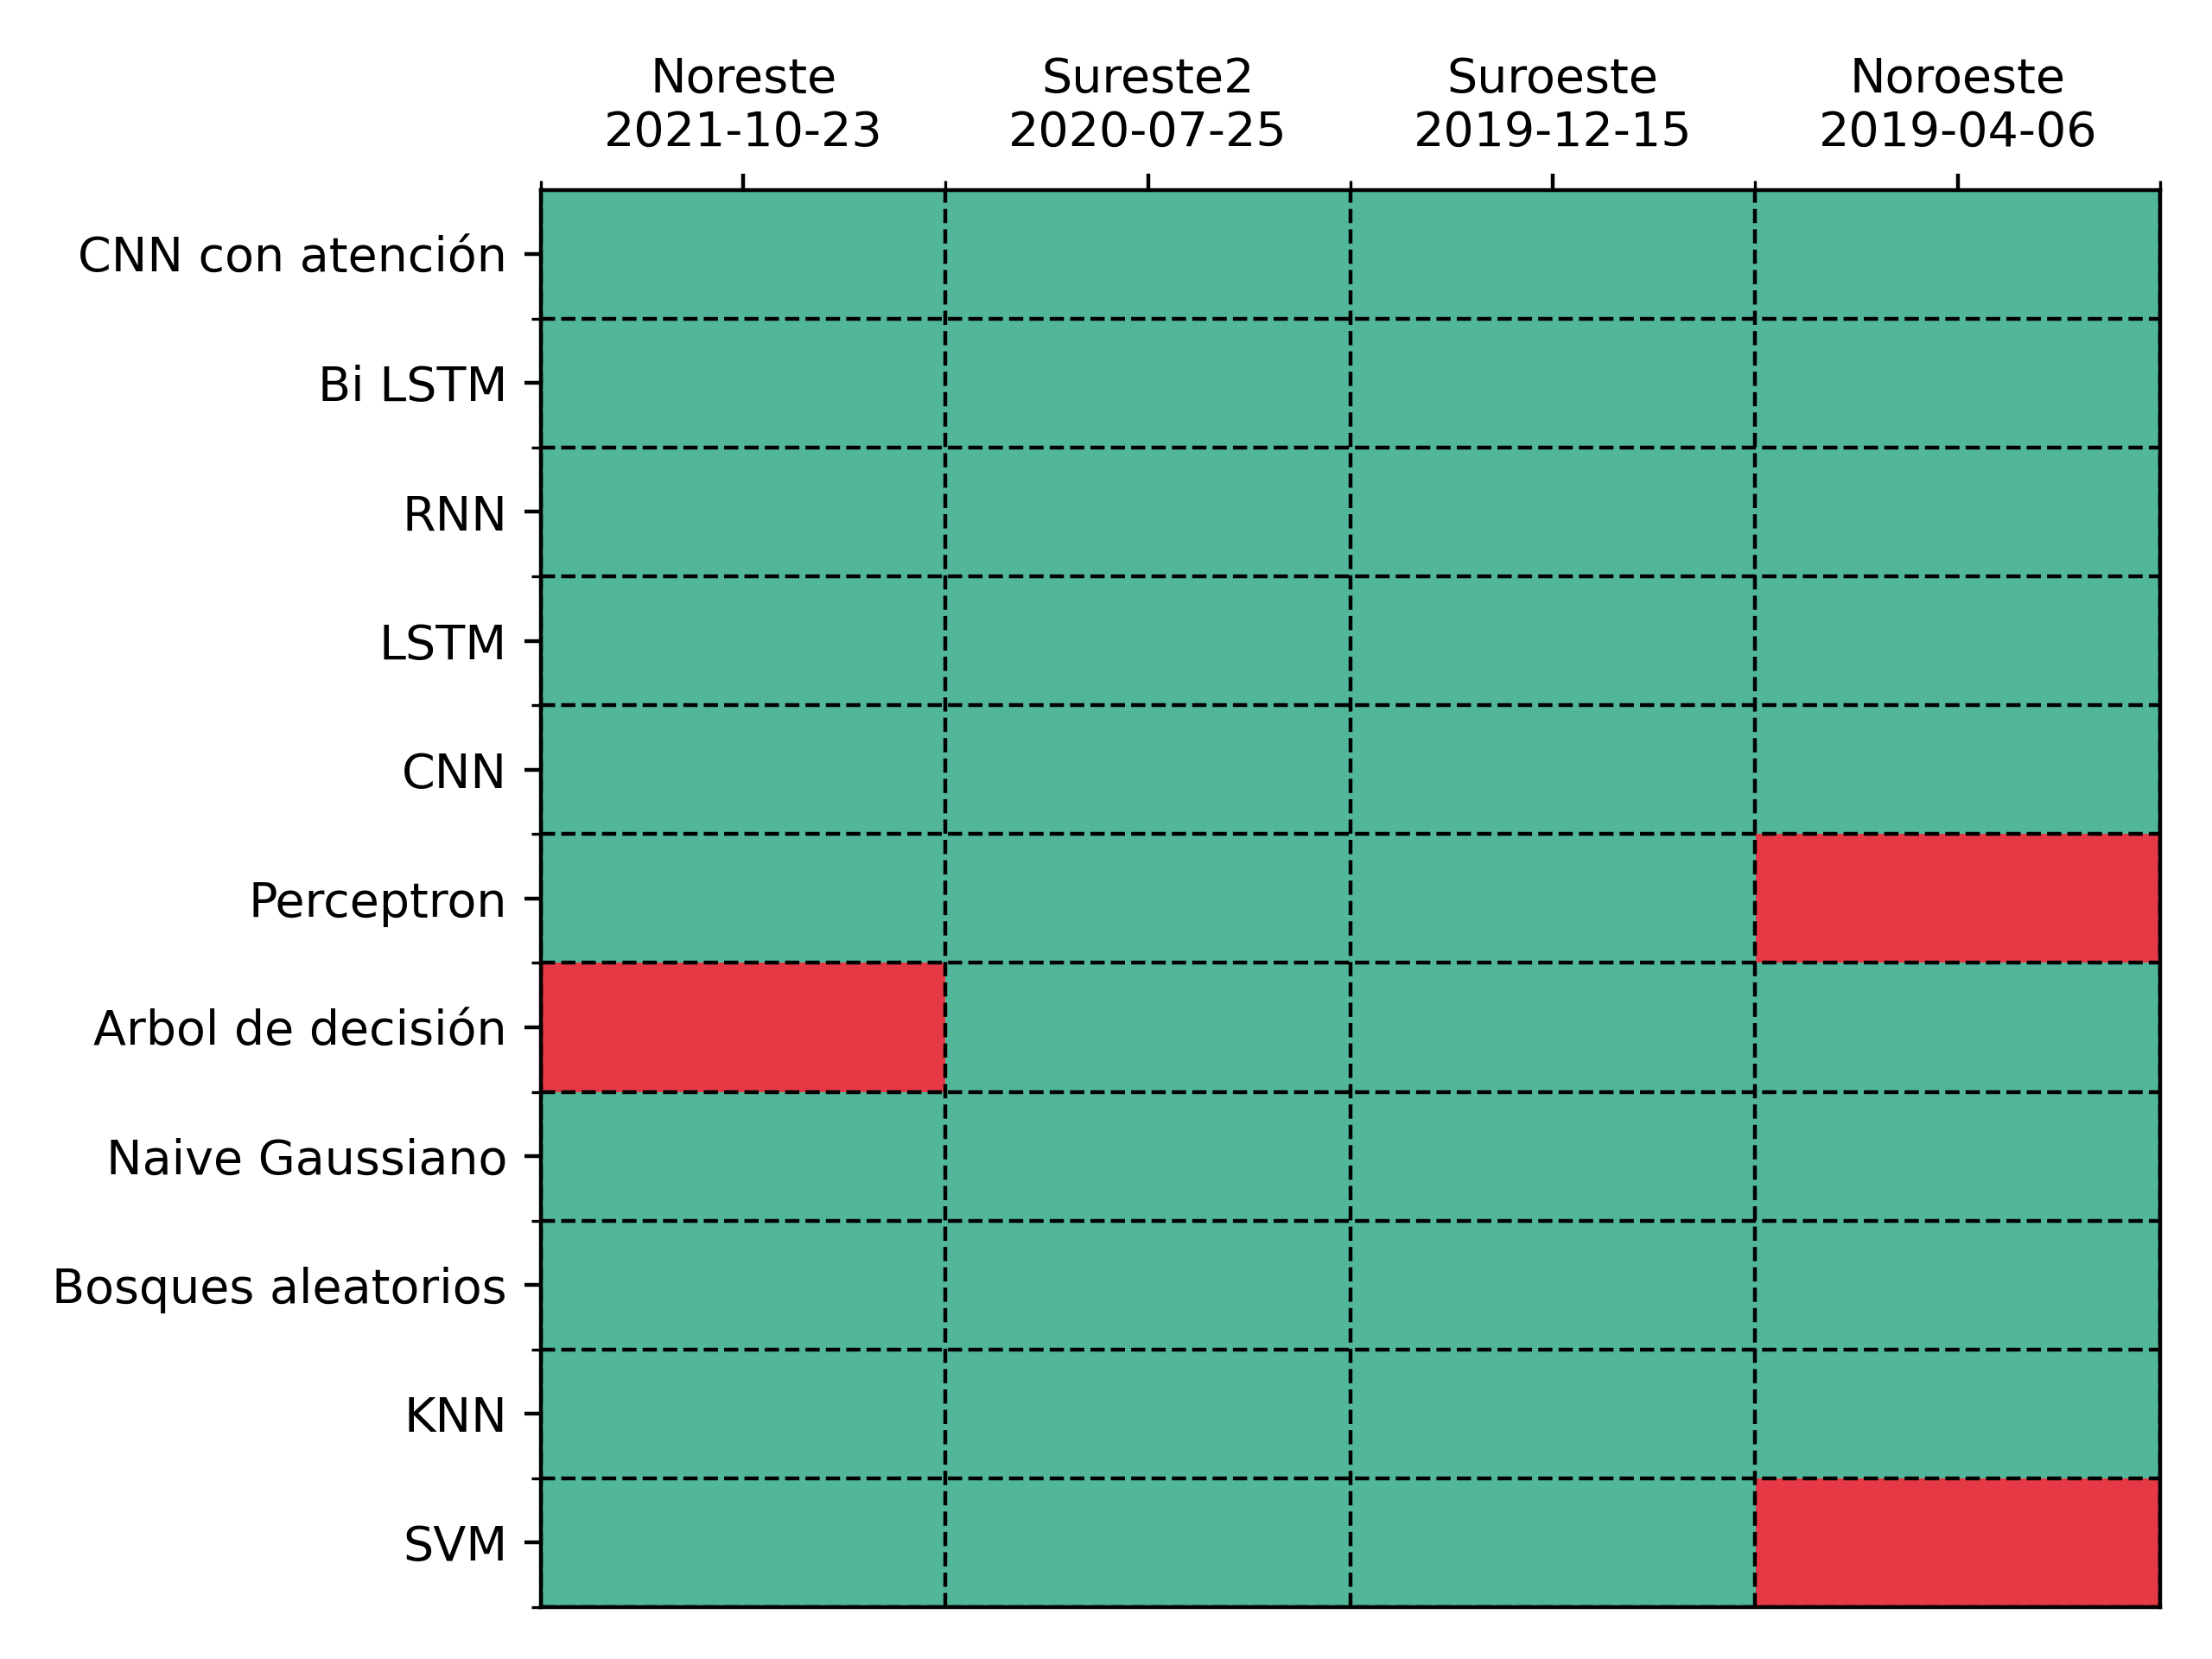
\includegraphics[width=10cm]{Graphics/Test_models.png}
	\caption{Resultados de la clasificación usando los modelos implementados para las fechas seleccionadas.}
	\label{fig:test_models}
\end{figure}
